
A density function (distribution) is a mapping from each element in an outcome space $x \in X$ to a number between 0 and 1.
This mapping is generally written as $p(x):=\PP(X=x), x \in X$ to denote the distribution over possible realizations $x$ of $X$.
$X$ may also denote a \textit{set} of random variables $X:=\{X_i\}_{i=1}^n$, where a draw from the distribution over $X$ results in a vector $x$. When $X$ follows the law defined by a specific $p(x)$, we say $X$ is a random variable with distribution $p(x)$.
The \textit{expectation} of a random variable $\EE[X]$ is the ``weighted average'' over all outcomes. For discrete variables (which will be our main focus with expectations), 
\begin{align}
\EE[X] = \sum_{x\in X} x\cdot p(x)
\end{align}
The properties of distributions below extend to measures of expectations among multiple variables, with some caveats mentioned in specific chapters as needed.

Over a set of random variables $X$ and $Y$, the distribution $p(x,y):= \PP(X=x,Y=y)$ is the \textit{joint} distribution over both variables $(X,Y)$. The \textit{marginal} distribution for $x$ is computed by ``summing out'' $y$, i.e.,
\begin{align}
p(x) = \PP(X=x) &= \sum_y \PP(X=x,Y=y) = \sum_y p(x,y) \\
&= \int p(x,y) dy
\end{align}
We say that the random variables $X$ and $Y$ are \textit{independent}
if their joint distribution is equal to the product of their marginals: $p(x,y) = p(x)p(y)$.
Intuitively, a draw from one distribution has no impact on the draw from the other.
In the case where the variables are \textit{dependent}, the distributions are linked.
The dependent draw is defined by the \textit{conditional} distribution $p(y|x)$.
Then, a joint distribution can factor as
an iterative draw first from $p(x)$ followed by from $p(y|x)$: $p(x,y) = p(x)p(y|x)$.
Importantly, this dependence is commutative:
it is also true that $p(x,y) = p(y)p(x|y)$.
When $p(y|x) = p(y)$, we say that $Y$ is independent of $X$.
This commutativity leads to the formulation of Bayes' Rule:
\begin{align}
    p(y|x) = \frac{p(x|y)p(y)}{p(x)}
\end{align}
This form is used throughout statistics and machine learning.
In most settings, we are interested in estimating some parameters $\theta$,
or distribution over parameters $p(\theta)$, given a distribution over data $p(x)$.
Applying Bayes' Rule:
\begin{align}
    p(\theta|x) = \frac{p(x|\theta)p(\theta)}{p(x)}
\end{align}
Where $p(x|\theta)$ is the \textit{likelihood} of observing the data $x$ given some parameter set,
$p(\theta)$ is the \textit{prior} assumption on the base distribution over parameters,
$p(x)$ is the marginal over all data (typically treated as a normalizing constant),
and $p(\theta|x)$ is the \textit{posterior} distribution over the parameters given some data.
Alternatively, we wish to update our estimation of the parameters $\theta$
from $p(\theta)$ to $p(\theta|x)$ given some observations $x$ that change our beliefs about the parameter space.
Maximum a posteriori (MAP) estimation attempts
to find the parameters that maximize this posterior,
using Bayes' rule for tractable computation and estimation.
\begin{align}\label{eq:map}
	\max_\theta p(\theta|x) = \max_\theta \frac{p(x|\theta)p(\theta)}{p(x)} =  \max_\theta p(x|\theta)p(\theta)
\end{align}
If we have some samples $\{x_i\}_{i=1}^n$ from the data distribution that comprise a dataset,
then we have the following equivalent log-transformed model:
\begin{align}
	\max_\theta \sum_{i=1}^n \log p(x_i|\theta) + \log p(\theta)
\end{align}
This is the canonical form used in most of machine learning:
generally associating a ``loss" or recovery term to the likelihood,
and a regularization to the prior.

\subsection{Conditional Independence} 
With three or more variables, independence relations among variables may be determined by which variables are being conditioned upon. 
\begin{definition}[Conditional Independence]\label{def:condindep}
For three random variables $X,Y,Z$, we say that 
$Y$ is \textit{conditionally independent} of $X$ given $Z$, written as $Y \indep X | Z$, if
\begin{align}
    p(y,x|z) = p(y|z)p(x|z).
\end{align}    
\end{definition}
Intuitively, once $Z$ is known, $X$ provides no additional information in predicting $Y$. This can also be written as $p(y|x,z)=p(y|z)$.

\paragraph{Graphs.}
With a larger number of variables, tracking independence relations can
become cumbersome with this notation.
\textit{Graphs} are commonly used in place.
Graphs $G$ are defined by their vertex and edge sets $G:=(E,V)$.
The vertices $V$ correspond to some random variables $X,Y,Z,\ldots$, or $X_1,\ldots,X_n$. 
An \textit{undirected} graph is one in which the existence of an edge $e_{ij}$ implies the existence of edge $e_{ji}$.
Within a \textit{probabilistic graphical model},
an edge $e_{ij}$ implies a \textit{conditional dependence}.
The omission of a particular edge thus has an explicit meaning:
\begin{align}
    e_{ij} \not\in E \iff X_i \indep X_j | X_{V\setminus(i,j)}
\end{align}
Where $V\setminus(i,j)$ is the rest of the variables in the set and graph.
A graph with these independence relations is also referred to as a Markov graph:
pairwise conditional independence relations imply
\textit{global} conditional independence relations:
for any sets of variables $A,B,C$, if $C$ ``separates'' $A$ and $B$, 
While directed graphs (Bayesian networks) are used and are of independent interest,
in this thesis we focus on undirected graphs.

\paragraph{Multivariate Gaussians.}
Extending the typical univariate Gaussian distribution
$p(x) = \frac{1}{\sqrt{2\pi\sigma^2}}e^{-(x-\mu)^2/2\sigma^2}$
defined by mean and variance parameters $\mu,\sigma^2$,
we have the following exponential density function
for multivariate Gaussian distributions over $n$ variables,
with realizations as the vector $\mathbf{x}:=[x_1,\ldots,x_n]^\top$:
\begin{align}\label{eq:mvgauss}
    p(x_1,\ldots,x_n) = \frac{1}{\sqrt{(2\pi)^n|\Sigma|}} \exp\left(\frac{1}{2}(\mathbf{x} - \mathbf{\mu})^\top \Sigma^{-1} (\mathbf{x} - \mathbf{\mu})\right)
\end{align}
Where $\mathbf{\mu}$ is the vector of means for each individual variable,
and $\Sigma$ is the $n\times n$ \textit{covariance} matrix
describing the second-order interactions among the variables. 
The tractability of both computing the density and estimating it
in typical likelihood estimation frameworks makes
the multivariate Gaussian a particular attractive prior used in many applications,
including estimating independence.
Specifically, 
\begin{theorem}\label{thm:mvnindep}
    Let $X$ be governed by a multivariate Gaussian as defined in \eqref{eq:mvgauss}. Then it holds that
    \begin{align}
        \Sigma_{ij} = 0 \iff X_i \indep X_j
    \end{align}
\end{theorem}
Complete independence among variables is often not possible and in most settings not valuable.
However, a more practical result for conditional independence exists.
\begin{theorem}\citep{lauritzen1996graphical}\label{thm:mvncondindep}
    Let $X$ be governed by a multivariate Gaussian as defined in \eqref{eq:mvgauss}, and $\Omega:=\Sigma^{-1}$ be the precision matrix.
    Then it holds that
    \begin{align}
        \Omega_{ij} = 0 \iff X_i \indep X_j | X_{\setminus(i,j)}
    \end{align}
\end{theorem}
This immediately yields that the precision matrix encodes the edges of the probabilistic graphical model over the variables.
Estimating these dependencies is thus equivalent to estimation of the precision matrix.
Further, if the precision matrix is sparse, we can  
derive dependencies between features when the data is high-dimensional and/or the number of measurements are small. 

\subsection{Estimating Parameters and Measures Over and Among Distributions}
Multivariate data analysis exploiting the conditional independence structure between features or covariates using 
undirected graphical models is now standard within any data analysis toolbox. 
When samples are drawn from a particular family of distributions, a number of methods exist to estimate the parameters that fit that data best. 
The estimation of a graphical model
has been extensively studied
and a rich literature is available describing 
its statistical and algorithmic properties \citep{koller2009probabilistic,jordan1998learning}. 
MAP estimation and maximum likelihood estimation as described above are typically used,
but in many cases their standard forms do not yield
parameters that reveal independence, i.e., it is often impossible for standard
methods to result in a parameter estimate of zero.

To determine the relationship among two random variables, measures such as the Pearson correlation coefficient, and Spearman and Kendall rank coefficients \citep{myers2013research} are frequently used, with values close to zero suggesting a low importance, and a value close to 1 suggesting perfect dependence. However,
these measures are only applicable with specific assumptions about the possible dependencies between the variables: Pearson coefficients can only identify linear dependencies, and rank coefficients typically fail with non-monotonic dependencies (e.g., periodic functions). These methods can be computed pairwise among all variables among a set of variables with size greater than 2, however, to estimate conditional dependencies typically requires the estimation of \textit{partial} coefficient measures.
Additionally, while results similar to Theorem~\ref{thm:mvncondindep} exist under specific assumptions ,
practical estimation does not often yield exact zeros,
and estimating all partial coefficients separately can be computationally heavy.

With some assumptions, \textit{sparse} recoveries are possible while estimating ALL conditional independencies. Following the results from multivariate Gaussians above,
a \textit{penalized} version of a maximum likelihood estimate can be recovered through the following \textit{graphical lasso} \citep{friedman2008sparse} formulation:
\begin{align}\label{eq:glasso}
    \hat{\Omega} = \min_{\Omega \succeq 0} \tr(\hat{\Sigma}\Omega) + \log|\Omega| + \lambda||\Omega||_1
\end{align}
With $\hat{\Sigma}$ being the sample covariance of the data samples, and $\lambda$ a penalization weight. The constraint $\Omega \succeq 0$ restricts the solution to be positive semi-definite: symmetric matrices with nonnegative eigenvalues. This $\ell_1$ penalization has been shown to be easy to compute, and a number of alternative versions have been proposed with varying theoretical properties and recovery guarantees~\citep{cai2011constrained,yuan2010high}.
Particularly interesting are extensions to \textit{nonparanormal} distributions, which allow for a much larger set of graphs to be estimated over other distributions via a rank covariance matrix, generalizing the pairwise rank and distance coefficients above \citep{liu2009nonparanormal,xue2012regularized}.

The distributional assumptions needed for all of these methods, however, are often completely unknown in practice, or the data represent highly complex densities and functions that cannot be represented by simple exponential families or rank-based measures.
Newer measures of \textit{nonparametric} estimations of dependence have been developed, such as distance correlation and kernel-based coefficients \citep{szekely2014partial,wang2015conditional,doran2014permutation}, but they tend to either only test for independence and not strength of functional relationship, or have complex instantations or asymptotic theories, making them difficult to deploy and rely upon in practice.
\begin{figure}
	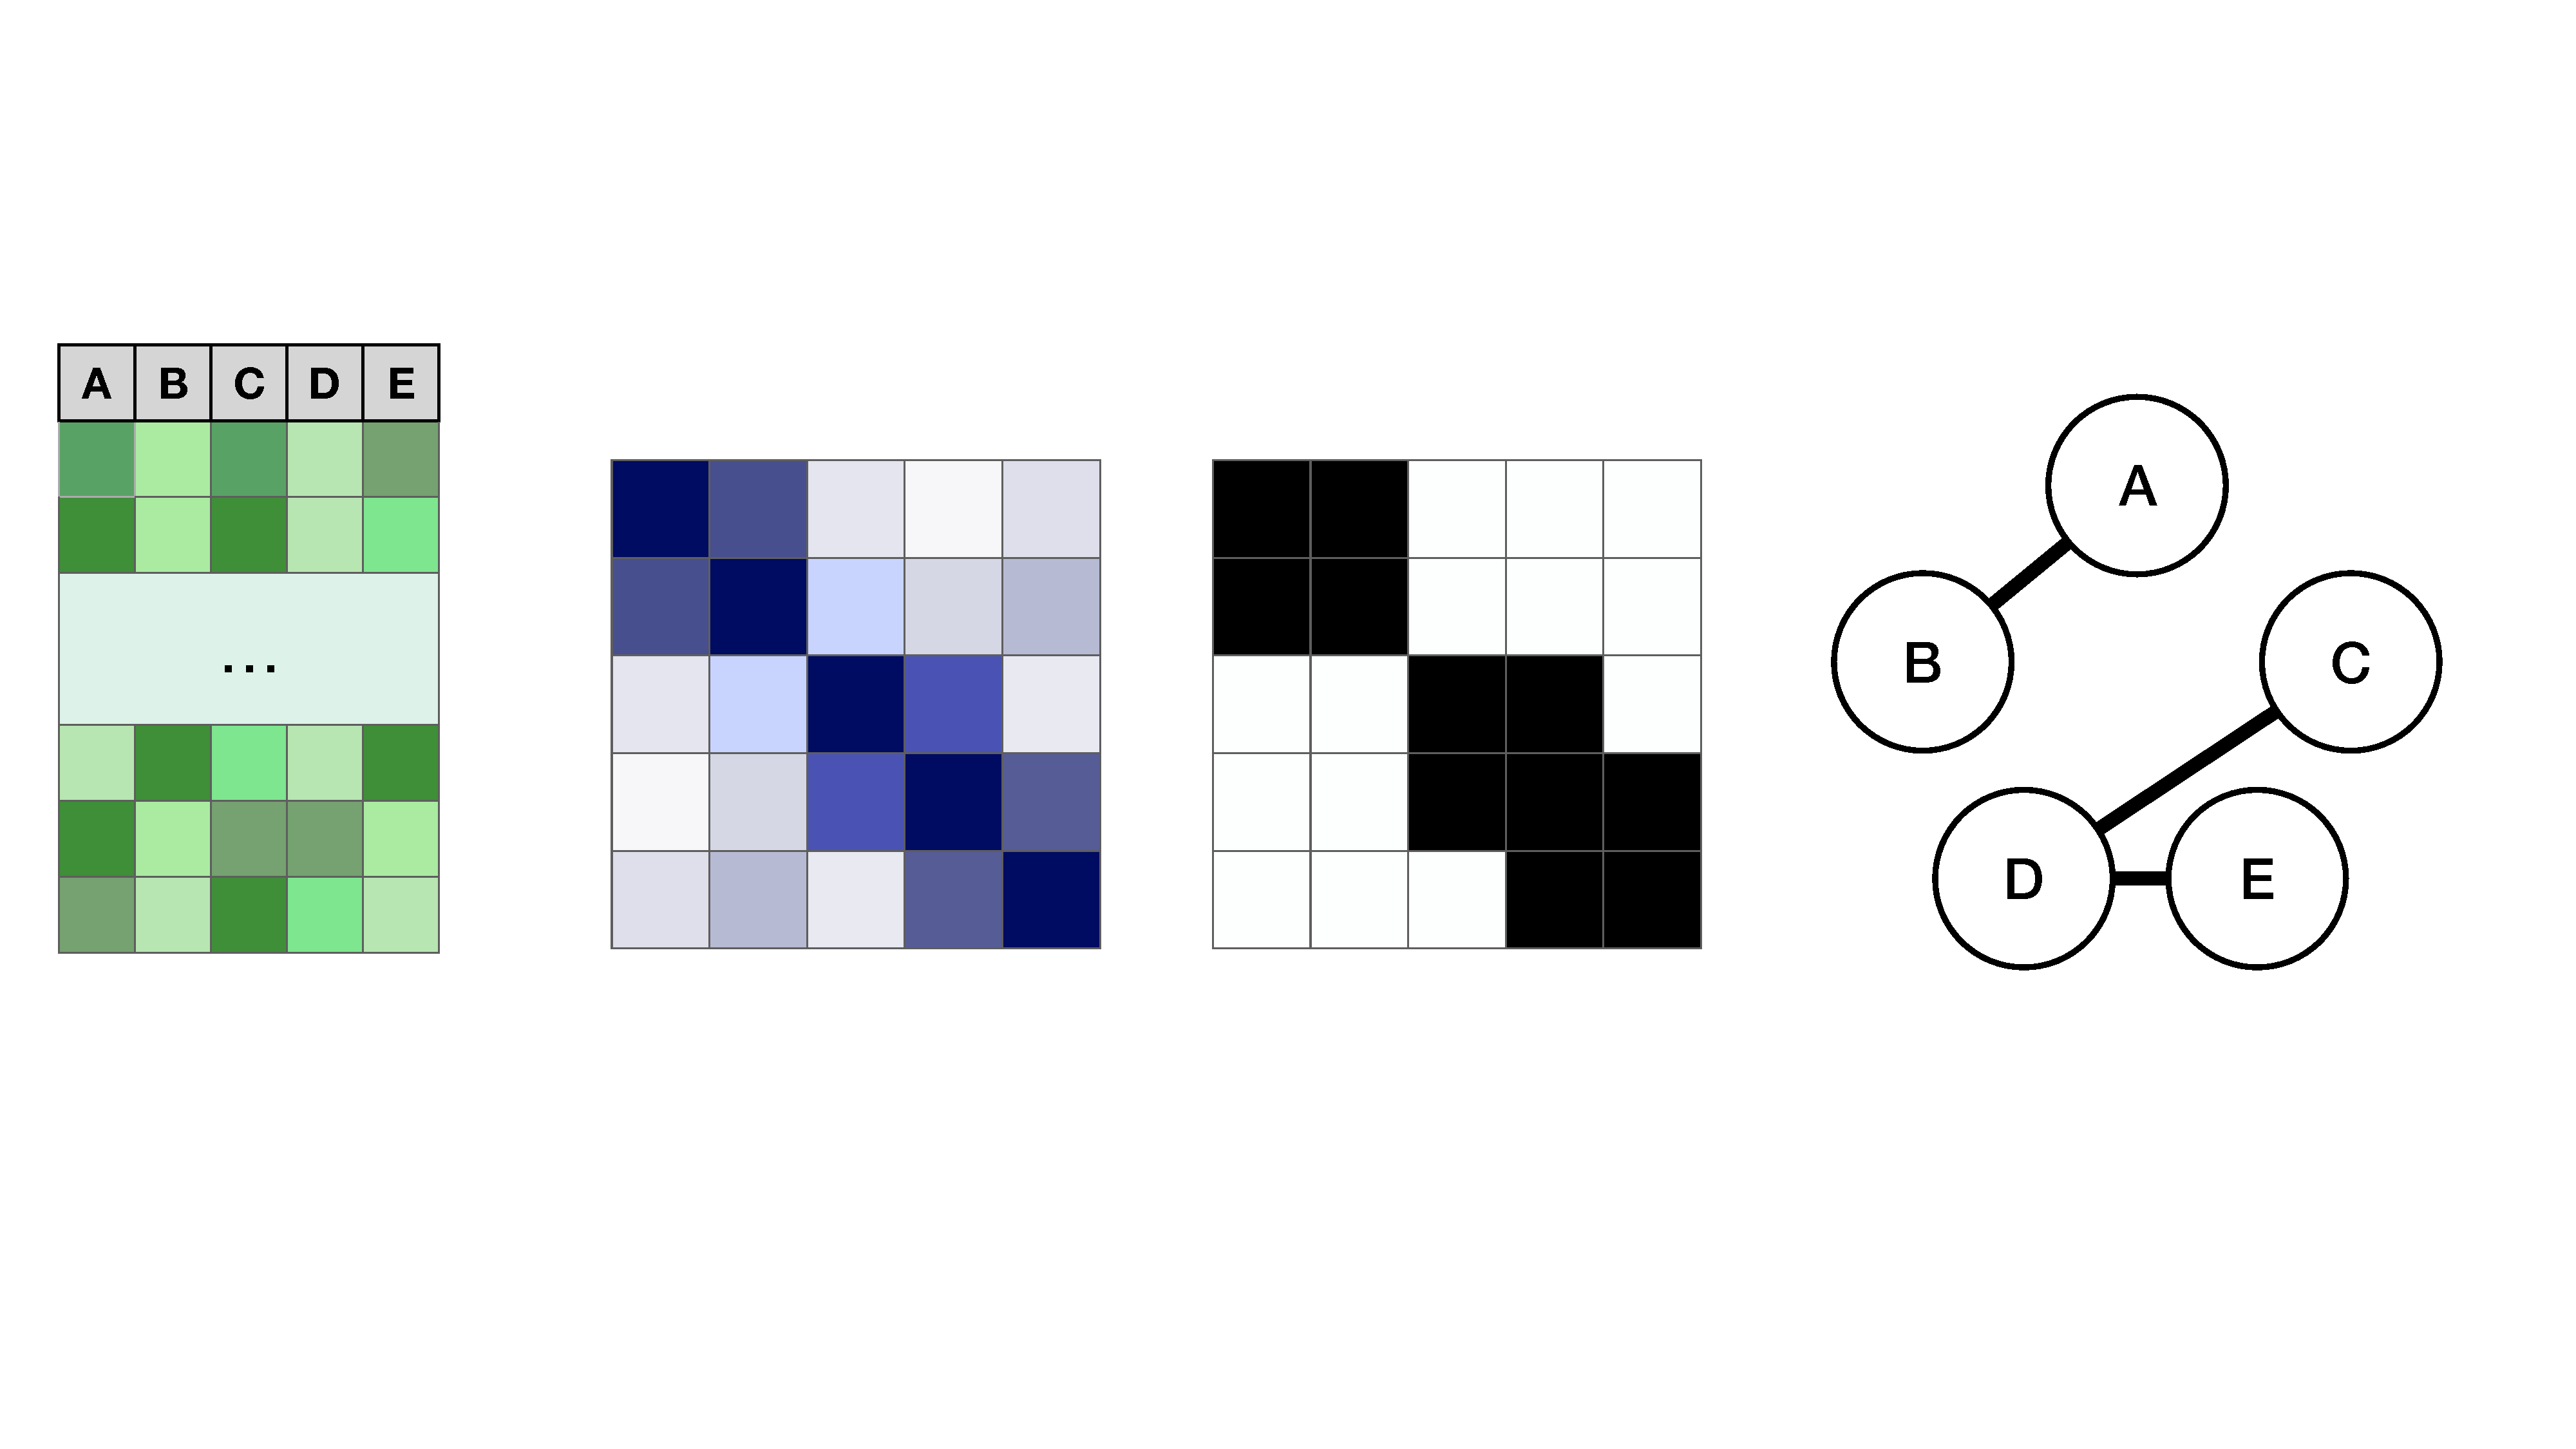
\includegraphics[width=\textwidth,trim={0 10cm 0 5cm},clip]{2_bknd/graphest.pdf}
	\caption[Graph estimation from data]{From data collected on various measures (left), we can compute a covariance matrix, estimate a sparse inverse, and recover the conditional independence relationships among measures (right).}
	\label{fig:graphest}
\end{figure}


A recent coefficient, the Chatterjee coefficient, has been demonstrated to have a number of desirable properties, and has been further developed into an elegant method for testing conditional independence~\citep{chatterjee2020new,codec}. 
Particularly,
no conditional densities need to be estimated,
it can be computed in $O(n\log n)$ time where $n$ is the number of data samples,
it asymptotically to 0 for conditional independence, and 1 for measurable functions,
and it requires \textit{absolutely no assumptions} on the law over the random variables.
For arbitrary variables random $X,Y,Z$, where $Y$ is univariate and $X,Z$ can be multivariate of any size, the conditional coefficient is given  by
\begin{align}\label{eq:contcodec}
    T(Y,X|Z) = \frac{\int\EE\left[\VAR(\PP(Y\geq t)|X,Z)|Z)\right]d\mu(t)}{\int\EE\left[\VAR(\II\{Y\geq t\}|Z\right] d\mu(t)}
\end{align}
with $\VAR(\cdot)$ denoting the variance over the random variable.
In Chapter~\ref{chap:lcodec} we will take advantage of these properties. Critically, without a specific procedure, identifying the conditioning set for a particular independence test is exponential. If we wish to find which variables $X_1,\ldots,X_n$ are sufficient for creating independence between some outcome $Y$ and the rest of the variables, na\"ively we would need to test all possible subsets.
An advantage of the coefficient of dependence in \cite{codec} is that it admits a linear time algorithm for iteratively building the sufficient set, naturally enabling an algorithm for constructing a Markov graph over the variables of interest.

\subsection{Hypothesis Testing}

Statistical hypothesis testing involves formally defining and testing a hypothesis about the world.
A prior ``null'' assumption is defined. The \textit{null} hypothesis, $H_0$
represents the default assumption or expectation
that there is no relationship or distinction among
the true population states,
whereas the \textit{alternative} hypothesis, $H_A$,
describes the world in which some hypothesized 
relationship or distinction does exist.
Testing proceeds by collecting observations
of the variables of interest,
computing a \textit{test statistic},
and comparing that statistic against
a prior \textit{null distribution}.
If the test statistic is larger
than a predefined critical value,
the null hypothesis is rejected:
there is reasonable evidence to suggest
the alternative may be true.
When we fail to reject the null,
there is insufficient evidence to support
the alternative claim.

The form of the test statistic and null distribution
are defined by the specific hypothesis being tested,
as well as the prior assumptions about the parameters
of interest and data collected.

\paragraph{Example: Testing a difference of means.} 
Say we have collected samples from two different groups,
representing the height of each person in the group.
Our task is to determine if the average height
of the two groups is significantly different from each other.
Na\"ively, we can compute the averages of the two groups and compare.
In practice these averages will never be equal, so how can we 
more rigorously determine if we should consider some measured difference
significant enough to say the groups are different?
We can set up the following hypothesis test.

Let $\mu_1$ be the true \textit{population mean} of group 1,
and $\mu_2$ the true population mean of group 2.
Our hypotheses are:
\begin{align}
H_0: \mu_1 = \mu_2 \qquad H_A: \mu_1 \neq \mu_2
\end{align}
Let us assume we have collected the same number of samples from each group,
$n$, and that the means of the collected samples are $\hat{\mu}_1$ and $\hat{\mu}_2$,
and the standard deviations are $s_1$ and $s_2$.
Then the test statistic
\begin{align}
t = \frac{\hat{\mu}_1 - \hat{\mu}_2}{\sqrt{\frac{s_1^2 + s_2^2}{n}}}
\end{align}
follows a $t$-distribution with $n-1$ degrees of freedom,
\textbf{if} there is no difference between the means.
Comparing the value of the measured statistic over the observed data
to the corresponding $t$-distribution allows
us to determine how likely or unlikely it is that 
our observation follows the law that the means are equal.
If we want our test to accurately identify
a difference between means 95\% of the time,
we can set our threshold $t^*$ (critical value) for rejecting the null
to be the point where $\PP(t \geq t^*) \geq 0.95$.

Importantly, the value of the $t$-statistic and corresponding
distribution and critical value are extremely
dependent on the number of samples $n$ acquired for the test.
As we will see, in cases where the number of samples is 
very small and our hypothesis describes 
a subtle difference between groups,
novel tests and procedures are necessary
to effectively identify those differences.

\subsubsection{Likelihood ratios and permutation testing}
Two challenges often appear in practice:
\textbf{(1)} An obvious test statistic may not exist,
and \textbf{(2)} the null distribution of that statistic
or the one chosen may not have a clear form.

In the case of large parametric models,
distributions over hundreds of parameters or more
become infeasible to compute in practice. In these
cases, the \textit{likelihood-ratio test} can be used.
With our posterior notation above, we have the following
test statistic for the null hypothesis $\theta\in\Theta_0, \Theta_0\subseteq\Theta$ and the alternative $\theta\in\Theta^C:=\Theta\setminus\Theta_0$:
\begin{align}\label{eq:lrt}
\lambda_{LR} = -2\text{ln}\left[ \frac{\sup_{\theta\in\Theta_0}p(x|\theta)}{\sup_{\theta\in\Theta} p(x|\theta)} \right]
\end{align}
The true power of the LRT statistic comes from two fundamental results.
First, the distribution of $\lambda_{LR}$
asymptotically approaches a $\chi^2$ distribution
with a fixed number of degrees of freedom,
enabling easy testing (Wilk's Theorem, \citep{wilks}).
And second,
the Neyman-Pearson lemma states
that this likelihood-ratio test is the 
most powerful $\alpha$ level test for this case~\citep{neymanpearson}.

When even a likelihood ratio cannot be constructed in this form,
a nonparametric test exists that may be used
for any statistic defined by the problem of interest.
Consider again a test of the form in~\eqref{eq:hyptest},
but where instead of the mean we have some arbitrary
statistic over our two groups.
A \textit{permutation test} comprises
of generating a null distribution through
resampling. By shuffling the data
and recomputing the statistic,
we can estimate the distribution of the
statistic if there were no difference among the groups.
This distribution can then be used
as the null distribution for checking
if the true group allocations result in a 
test statistic significantly different
from the null distribution.

These ideas will be used to construct
and evaluate 
hypothesis tests in Chapter~\ref{chap:covtraj},
as well as in subsequent work building upon
those results.